\chapter{Geophysics Interferometer (GIF)}



\section{Overview} 
\subsection{Laser Strainmeter gor Geophysics}
\subsection{Motivation in GW detectors}


\section{Working Principle}

\subsection{Asynmetric Michelson Interferometer}
\begin{eqnarray}
  \phi = 2\pi\frac{2(l_x-l_y)}{\lambda}\sim4\pi\frac{l_x}{\lambda}
\end{eqnarray}

\begin{eqnarray}
  |d\phi| = 4\pi\frac{l_x}{\lambda}\left( \left|\frac{d\lambda}{\lambda}\right| + \left|\frac{dl_x}{l_x}\right| \right)
\end{eqnarray}


\subsection{Response to the seismic strain}
\begin{figure}[h]
  \begin{center}
    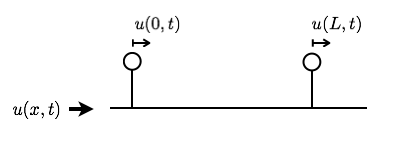
\includegraphics[width=10.0cm]{./img_chap4/img410.png}
    \caption{The displacements of the two points which are sparated L in X axis. }
  \end{center}
\end{figure}

The response of the strainmeter to seismic waves have characteristics of the low pass filter. To calculate this response, it is assumed that the plane seismic waves which displacement $u(x,t)$ is represented as $u(x,t)=u_0e^{i(\omega{t}-kx)}$ with angular frequency of $\omega$ and wave number of $k$, propagate along with the direction of the base-line of the strainmeter. The length fluctuation between two mirrors sparated with $L$ can be expressed as 
\begin{eqnarray}
  \Delta{L(t)} &\equiv& u(0,t) - u(L,t) \\
  &=& u(0,t) - u(0,t-\tau), \label{eq:chap4_10}
\end{eqnarray}
where $\tau=L/v$ is the time delay. 
The transfer function from the displacement to the length fluctuation is
\begin{eqnarray}
  H_{\mathrm{disp}}(s) \equiv \frac{\Delta{L(s)}}{u(s)} = 1 - \mathrm{exp}(-\tau{s})
\end{eqnarray}

Because the strain amplitude $\epsilon(x,t)$ is defined as $\epsilon(x,t)\equiv\frac{du}{dx}$, the strain
\begin{eqnarray}
  \epsilon(x,t) \equiv \frac{du}{dx} &=& \frac{du}{dt} \frac{dt}{dx}\\
  &=& {u(x,t)}^{\prime}\frac{1}{v}
\end{eqnarray}


Therefore, the response of the strainmter to the seismic strain is given

\begin{eqnarray}
  H_{\mathrm{strain}}(s) \equiv \frac{\Delta{L(s)}}{\epsilon(s)} = \frac{\Delta{L(s)}}{\frac{s}{v}u(s)} = \left(1 - \mathrm{exp}(-\tau{s})\right) \frac{v}{s}
\end{eqnarray}



\begin{figure}[h]
  \begin{center}
    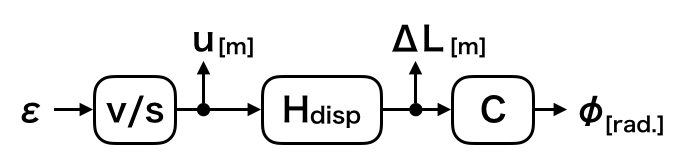
\includegraphics[width=10.0cm]{./img_chap4/img411.png}
    \caption{}
  \end{center}
\end{figure}


\begin{figure}[h]
  \begin{center}
    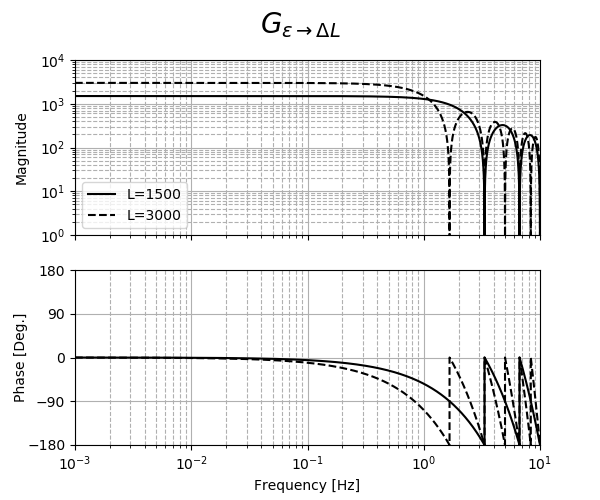
\includegraphics[width=12.0cm]{./img_chap4/img412.png}
    \caption{}
  \end{center}
\end{figure}


\subsection{Signal Detection Scheme}
\subsubsection{Quadrature Phase Detection}


\subsection{Noise}
どういうノイズが原理的に存在するか述べる。空気ゆらぎ、周波数雑音を述べる。




\section{Optics} %光学系
どうやって実際の干渉計を構築しているか述べる。
\subsection{Mode Matching Optics}
どういうモードマッチをして干渉計として光を干渉させているか述べる。
\subsection{Frequency Stabilized Laser}
どういう制御をして周波数安定をしているか述べる。
\subsection{Core Optics}
\subsubsection{Beam Splitter}
どういうミラーを使っているか述べる。
\subsubsection{Corner Cube}
どういうミラーを使っているか述べる。大きさとか表面の精度とか。




\section{Data Aquisition System}
\subsection{...}




\section{Summary of the Chapter} %章のまとめ
本章で述べたパラメータを表にまとめる。
